% Options for packages loaded elsewhere
\PassOptionsToPackage{unicode}{hyperref}
\PassOptionsToPackage{hyphens}{url}
%
\documentclass[
  ignorenonframetext,
]{beamer}
\usepackage{pgfpages}
\setbeamertemplate{caption}[numbered]
\setbeamertemplate{caption label separator}{: }
\setbeamercolor{caption name}{fg=normal text.fg}
\beamertemplatenavigationsymbolshorizontal
% Prevent slide breaks in the middle of a paragraph
\widowpenalties 1 10000
\raggedbottom
\setbeamertemplate{part page}{
  \centering
  \begin{beamercolorbox}[sep=16pt,center]{part title}
    \usebeamerfont{part title}\insertpart\par
  \end{beamercolorbox}
}
\setbeamertemplate{section page}{
  \centering
  \begin{beamercolorbox}[sep=12pt,center]{part title}
    \usebeamerfont{section title}\insertsection\par
  \end{beamercolorbox}
}
\setbeamertemplate{subsection page}{
  \centering
  \begin{beamercolorbox}[sep=8pt,center]{part title}
    \usebeamerfont{subsection title}\insertsubsection\par
  \end{beamercolorbox}
}
\AtBeginPart{
  \frame{\partpage}
}
\AtBeginSection{
  \ifbibliography
  \else
    \frame{\sectionpage}
  \fi
}
\AtBeginSubsection{
  \frame{\subsectionpage}
}

\usepackage{amsmath,amssymb}
\usepackage{lmodern}
\usepackage{iftex}
\ifPDFTeX
  \usepackage[T1]{fontenc}
  \usepackage[utf8]{inputenc}
  \usepackage{textcomp} % provide euro and other symbols
\else % if luatex or xetex
  \usepackage{unicode-math}
  \defaultfontfeatures{Scale=MatchLowercase}
  \defaultfontfeatures[\rmfamily]{Ligatures=TeX,Scale=1}
\fi
\usetheme[]{Antibes}
\usecolortheme{default}
% Use upquote if available, for straight quotes in verbatim environments
\IfFileExists{upquote.sty}{\usepackage{upquote}}{}
\IfFileExists{microtype.sty}{% use microtype if available
  \usepackage[]{microtype}
  \UseMicrotypeSet[protrusion]{basicmath} % disable protrusion for tt fonts
}{}
\makeatletter
\@ifundefined{KOMAClassName}{% if non-KOMA class
  \IfFileExists{parskip.sty}{%
    \usepackage{parskip}
  }{% else
    \setlength{\parindent}{0pt}
    \setlength{\parskip}{6pt plus 2pt minus 1pt}}
}{% if KOMA class
  \KOMAoptions{parskip=half}}
\makeatother
\usepackage{xcolor}
\newif\ifbibliography
\setlength{\emergencystretch}{3em} % prevent overfull lines
\setcounter{secnumdepth}{-\maxdimen} % remove section numbering


\providecommand{\tightlist}{%
  \setlength{\itemsep}{0pt}\setlength{\parskip}{0pt}}\usepackage{longtable,booktabs,array}
\usepackage{calc} % for calculating minipage widths
\usepackage{caption}
% Make caption package work with longtable
\makeatletter
\def\fnum@table{\tablename~\thetable}
\makeatother
\usepackage{graphicx}
\makeatletter
\def\maxwidth{\ifdim\Gin@nat@width>\linewidth\linewidth\else\Gin@nat@width\fi}
\def\maxheight{\ifdim\Gin@nat@height>\textheight\textheight\else\Gin@nat@height\fi}
\makeatother
% Scale images if necessary, so that they will not overflow the page
% margins by default, and it is still possible to overwrite the defaults
% using explicit options in \includegraphics[width, height, ...]{}
\setkeys{Gin}{width=\maxwidth,height=\maxheight,keepaspectratio}
% Set default figure placement to htbp
\makeatletter
\def\fps@figure{htbp}
\makeatother

\logo{
\includegraphics[width=2cm]{udem.png}}
\usepackage{copyrightbox}
\makeatletter
\makeatother
\makeatletter
\makeatother
\makeatletter
\@ifpackageloaded{caption}{}{\usepackage{caption}}
\AtBeginDocument{%
\ifdefined\contentsname
  \renewcommand*\contentsname{Table of contents}
\else
  \newcommand\contentsname{Table of contents}
\fi
\ifdefined\listfigurename
  \renewcommand*\listfigurename{List of Figures}
\else
  \newcommand\listfigurename{List of Figures}
\fi
\ifdefined\listtablename
  \renewcommand*\listtablename{List of Tables}
\else
  \newcommand\listtablename{List of Tables}
\fi
\ifdefined\figurename
  \renewcommand*\figurename{Figure}
\else
  \newcommand\figurename{Figure}
\fi
\ifdefined\tablename
  \renewcommand*\tablename{Table}
\else
  \newcommand\tablename{Table}
\fi
}
\@ifpackageloaded{float}{}{\usepackage{float}}
\floatstyle{ruled}
\@ifundefined{c@chapter}{\newfloat{codelisting}{h}{lop}}{\newfloat{codelisting}{h}{lop}[chapter]}
\floatname{codelisting}{Listing}
\newcommand*\listoflistings{\listof{codelisting}{List of Listings}}
\makeatother
\makeatletter
\@ifpackageloaded{caption}{}{\usepackage{caption}}
\@ifpackageloaded{subcaption}{}{\usepackage{subcaption}}
\makeatother
\makeatletter
\@ifpackageloaded{tcolorbox}{}{\usepackage[many]{tcolorbox}}
\makeatother
\makeatletter
\@ifundefined{shadecolor}{\definecolor{shadecolor}{rgb}{.97, .97, .97}}
\makeatother
\makeatletter
\makeatother
\ifLuaTeX
  \usepackage{selnolig}  % disable illegal ligatures
\fi
\IfFileExists{bookmark.sty}{\usepackage{bookmark}}{\usepackage{hyperref}}
\IfFileExists{xurl.sty}{\usepackage{xurl}}{} % add URL line breaks if available
\urlstyle{same} % disable monospaced font for URLs
\hypersetup{
  pdftitle={Reproducible papers in the life sciences using R},
  hidelinks,
  pdfcreator={LaTeX via pandoc}}

\title{Reproducible papers in the life sciences using R}
\author{Ariel Mundo Ortiz}
\date{CANSSI Statistical Software Conference\\
November 10, 2022}
\institute{Université de Montréal\\
\strut \\
@amundortiz (Twitter)\\
@aimundo (Mastodon)}

\begin{document}
\frame{\titlepage}
\ifdefined\Shaded\renewenvironment{Shaded}{\begin{tcolorbox}[breakable, enhanced, borderline west={3pt}{0pt}{shadecolor}, sharp corners, boxrule=0pt, interior hidden, frame hidden]}{\end{tcolorbox}}\fi

\begin{frame}[fragile]{Introduction}
\protect\hypertarget{introduction}{}
\begin{itemize}[<+->]
\item
  \texttt{RMarkdown} is a powerful tool to create reproducible papers
\item
  However, R is rarely used in the life sciences as a default method to
  create papers
\item
  \color{red}{Why?}
\end{itemize}
\end{frame}

\begin{frame}{Reasons}
\protect\hypertarget{reasons}{}
\begin{itemize}[<+->]
\tightlist
\item
  ``R is just for Stats''
\item
  ``There is a learning curve''
\item
  \textbf{``I can't create figures for publication''}
\end{itemize}
\end{frame}

\begin{frame}{The Problem}
\protect\hypertarget{the-problem}{}
\begin{itemize}[<+->]
\tightlist
\item
  Papers in the life sciences usually require figures where the
  following are combined:

  \begin{itemize}[<+->]
  \tightlist
  \item
    Images from cells/tissues
  \item
    Figures that summarize data
  \item
    Figures that present statistical analyses (with ``p-values'')
  \end{itemize}
\end{itemize}
\end{frame}

\begin{frame}{The Problem}
\protect\hypertarget{the-problem-1}{}
\begin{figure}
\centering
\caption{A typical figure}
\copyrightbox[b]{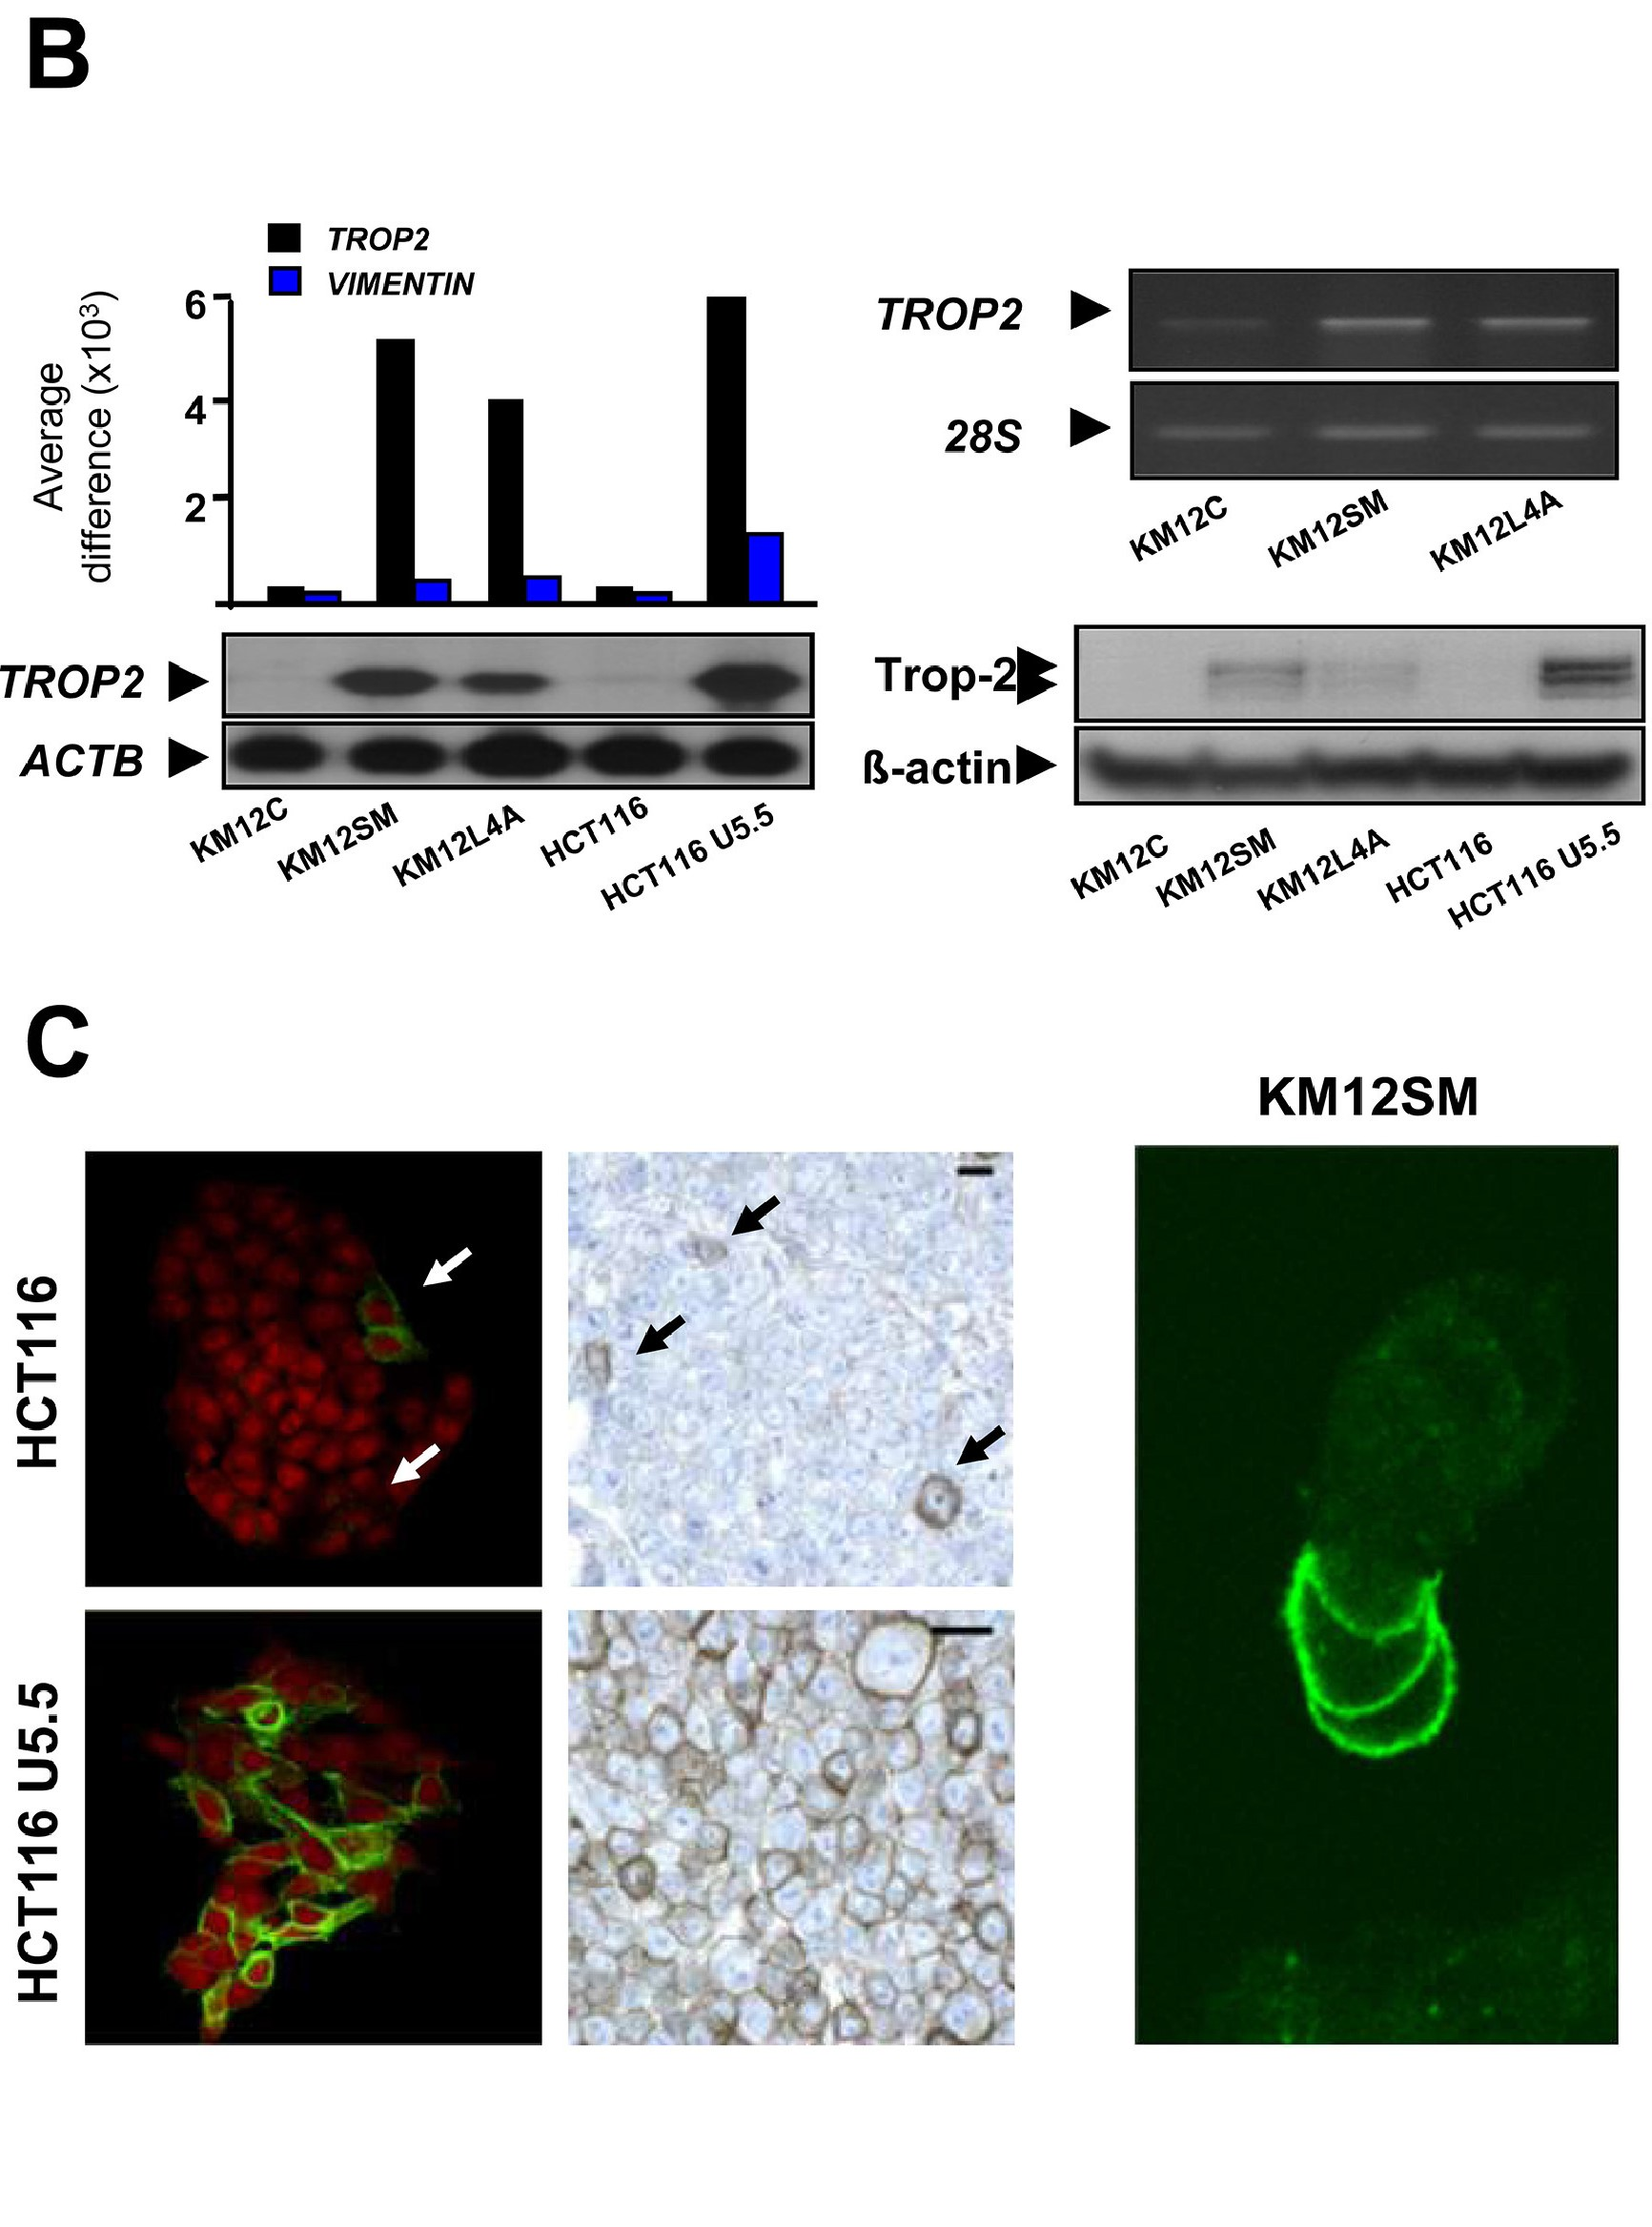
\includegraphics[width=2.5cm]{figure.jpg}}
                {\tiny{Guerra et al.} \textit{Neoplasia} \textbf{2021}}
    \end{figure}

\begin{itemize}[<+->]
\item
  \color{red}{Can figures like this be created using `RMarkdown`?}
\end{itemize}
\end{frame}

\begin{frame}{The Solution}
\protect\hypertarget{the-solution}{}
\begin{itemize}[<+->]
\item
  Yes, we can create figures like this using R!
\item
  We will need to use a combination of packages to achieve this
\end{itemize}

\begin{figure}
\centering
\caption{The packages}
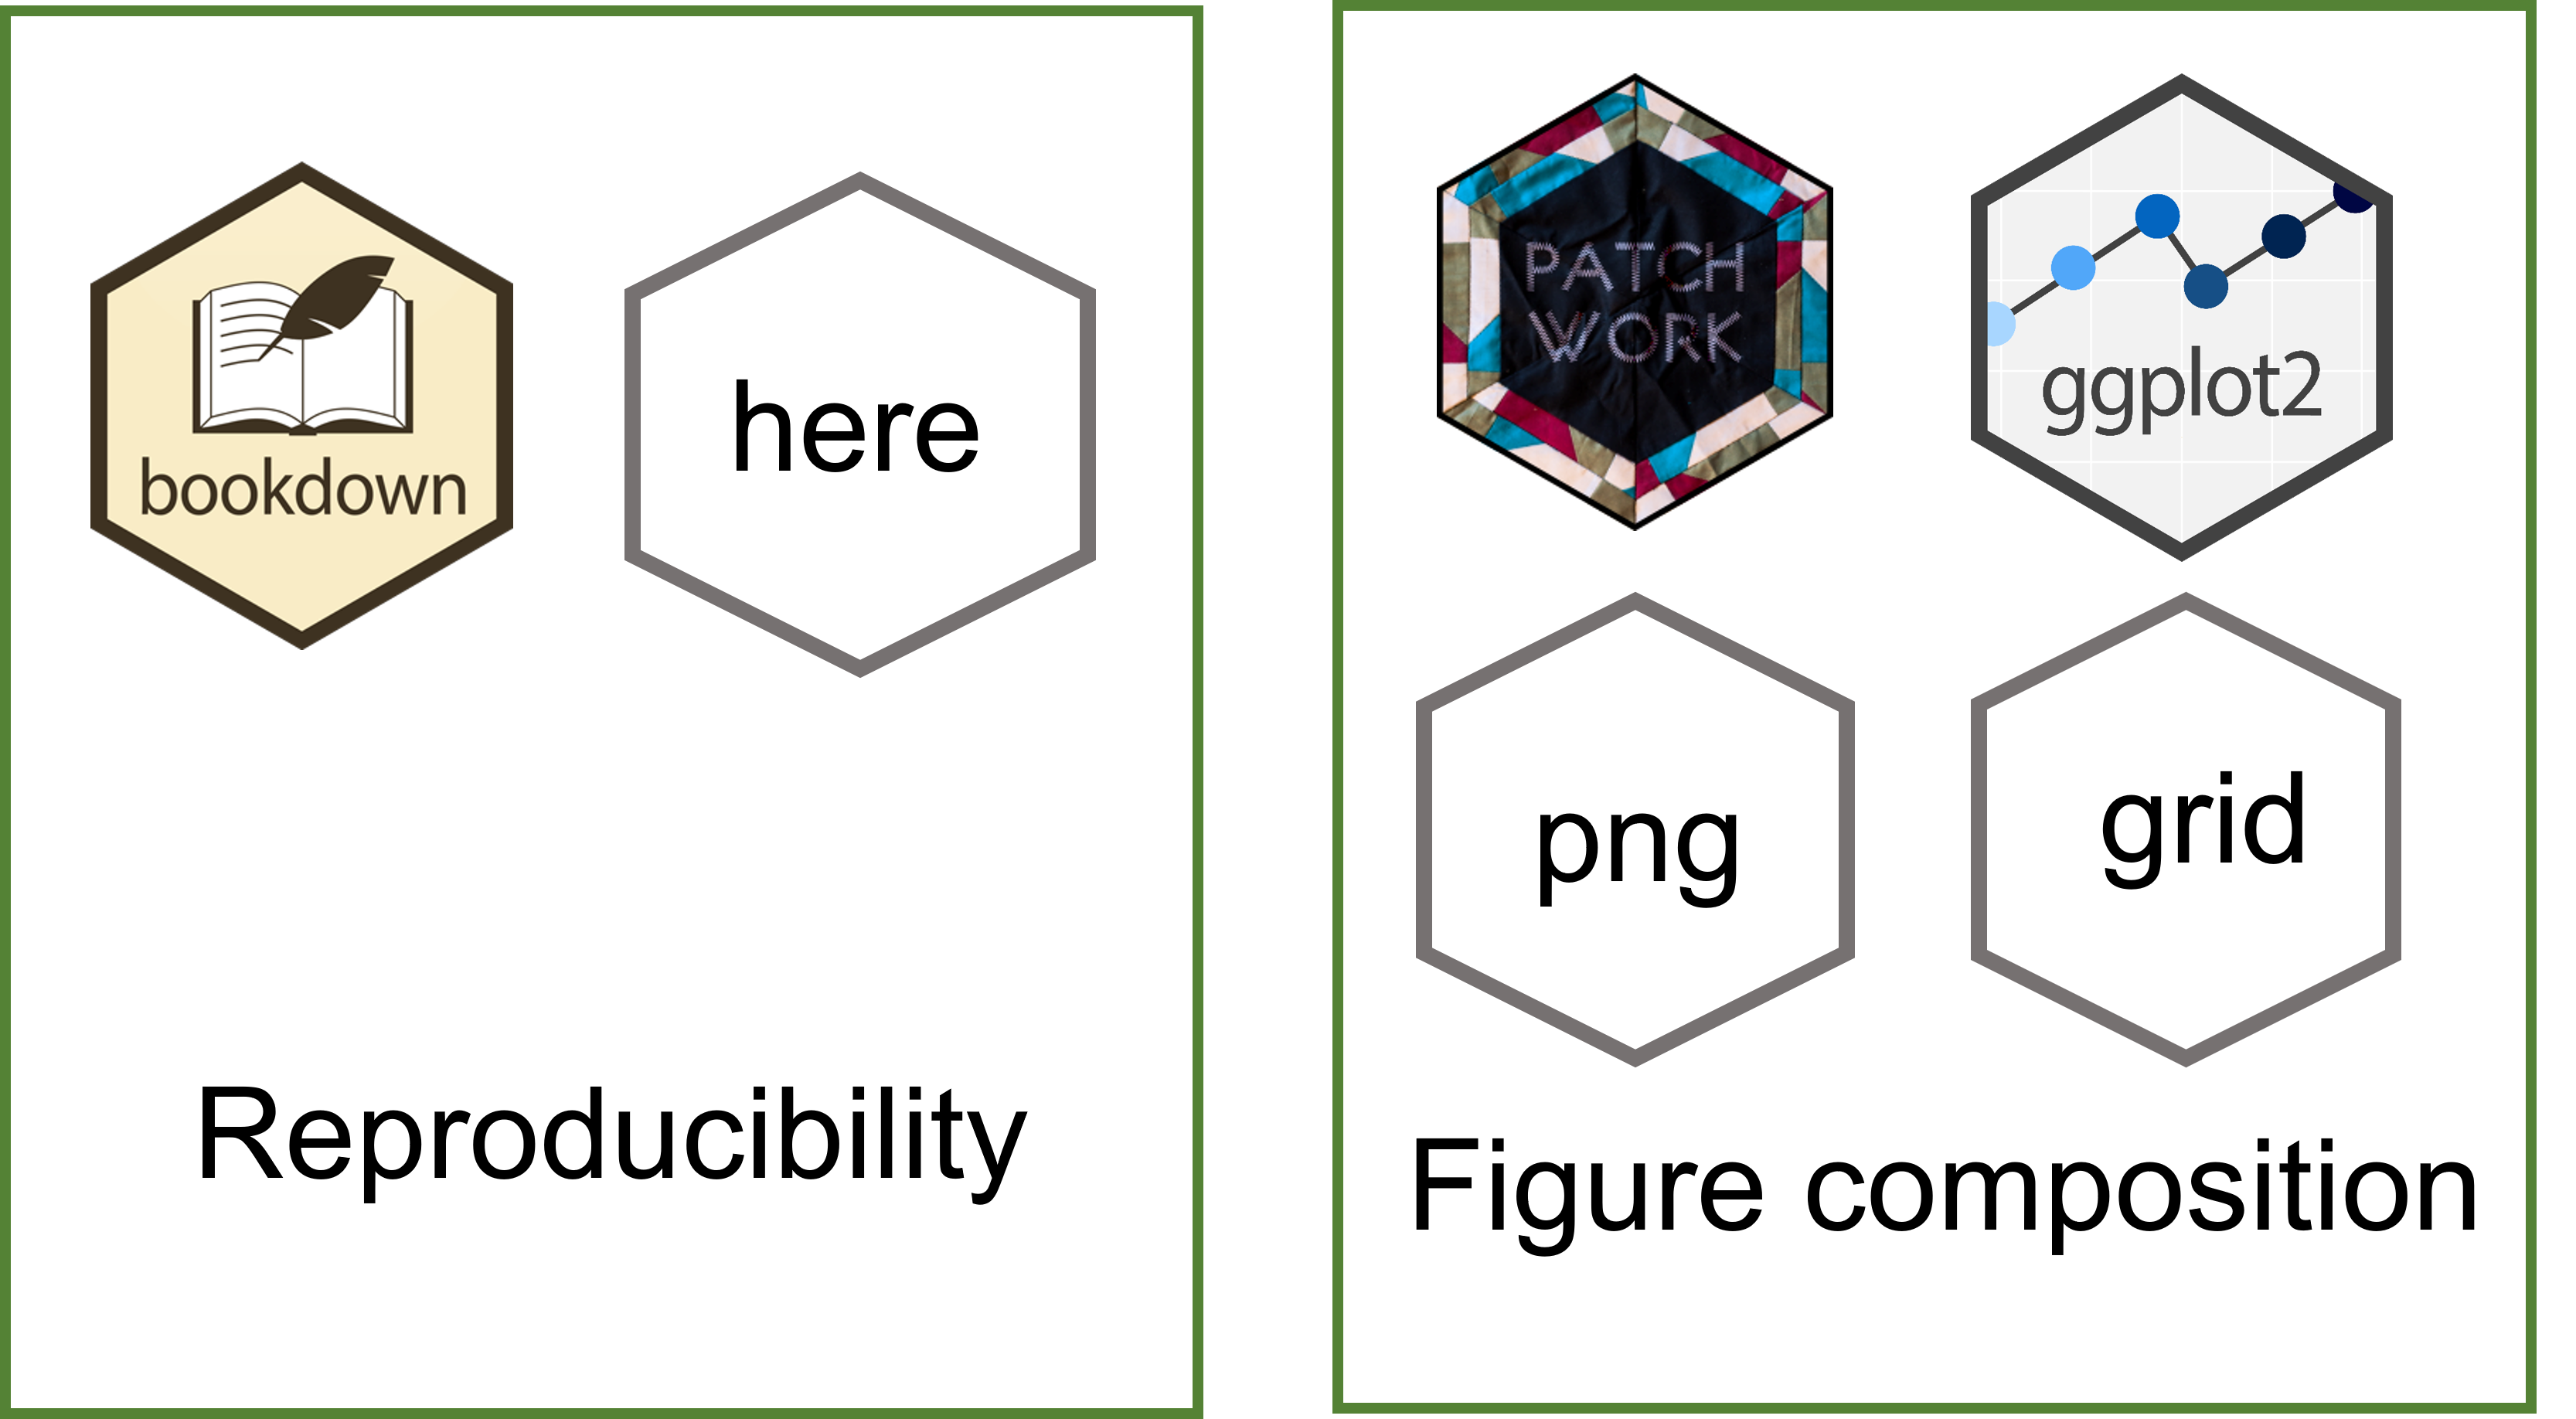
\includegraphics[width=6cm]{R_packages.png}
\end{figure}
\end{frame}

\begin{frame}[fragile]{The Solution}
\protect\hypertarget{the-solution-1}{}
\begin{itemize}[<+->]
\tightlist
\item
  \{bookdown\} allows to create a reproducible paper:

  \begin{itemize}[<+->]
  \tightlist
  \item
    Each section of the paper: (Materials and Methods, Results, etc.) is
    in a separate \texttt{Rmd} file
  \item
    More details can be found in \url{https://bookdown.org/}
  \end{itemize}
\item
  \{here\} allows to easily call scripts within the document (we will
  look at this later)
\end{itemize}
\end{frame}

\begin{frame}[fragile]{The Solution}
\protect\hypertarget{the-solution-2}{}
\begin{itemize}[<+->]
\tightlist
\item
  Let's think about a typical scenario, where you:

  \begin{itemize}[<+->]
  \item
    Have written your paper sections (Methods, Results, etc) each
    section is in a \texttt{Rmd} file
  \item
    Have some images
  \item
    Have some data that needs to be analyzed
  \item
    Want to create a composite figure of images/data analysis
  \item
    \textbf{For the sake of time, I will focus on the image
    composition/data analysis part}
  \end{itemize}
\end{itemize}
\end{frame}

\begin{frame}[fragile]{A Handy Script}
\protect\hypertarget{a-handy-script}{}
\begin{itemize}[<+->]
\tightlist
\item
  We can read the images (in PNG format), get the data, do the analysis
  and create the figure in a single script!

  \begin{itemize}[<+->]
  \tightlist
  \item
    Reading the images is achieved by \texttt{grid} and \texttt{png}
  \item
    \texttt{ggplot2} creates the plot of our analysis
  \item
    \texttt{patchwork} allows us to assemble everything
  \end{itemize}
\end{itemize}
\end{frame}



\end{document}
